\documentclass[10pt,a4paper]{extarticle}
\usepackage{geometry}
\usepackage{amsmath}
\usepackage{amsfonts}
\usepackage{amssymb}
\usepackage{isotope}
\usepackage{units}
\usepackage{nicefrac}
\usepackage{graphicx}

% Adjust page margins
\geometry{
textwidth = 15.6cm,
textheight = 24.7cm,
}
\pagestyle{empty}
\begin{document}
\section*{Vorbesprechung}

\subsection*{Einleitung}
\begin{itemize}
\item Welchen Versuch führen wir heute durch?
\item Was ist das Ziel des Versuchs? Was wollen wir in dem Versuch machen?
\item Wozu benötigt man kalte Atome?
\end{itemize}

\subsection*{Rubidium}
\begin{itemize}
\item Mit welchem Element arbeiten wir? Mit welchem Isotop arbeiten wir? 
\item Welche Wellenlänge benötigen wir ungefähr? 
\item Niveaustruktur \isotope[85]{Rb}, Kernspin $I=\frac{5}{2}$ \\ 
Grundzustand: $5^2\rm{S}_{1/2}$ ($n=5$, $S=\frac{1}{2}$, $L=0$ $\Rightarrow$ $J=\frac{1}{2}$) \\
angeregter Zustand: $L=1 \Rightarrow$ $5^2\rm{P}_{1/2}$($J=\frac{1}{2}$; D2-Linie) oder $5^2\rm{P}_{3/2}$ ($J=\frac{3}{2}$; D1-Linie) \\
Hyperfeinstrukturaufspaltung wegen Entartung des Gesamtdrehimpuls: $|J-I|<F<J+I$ \\
Natürliche Linienbreite  $\Gamma=2\pi\cdot\unit[6]{MHz} =1/\tau$ mit  $\tau=\unit[26]{ns}$ Lebensdauer
\end{itemize}

\subsection*{Laser und Laserstabilisierung:}
\begin{itemize}
\item Diodenlaser mit externem Resonator (Littrow-Anordnung und Interferenzfilter);
\item Laserschutz: Schutzbrille; Reflektierende Gegenstände ausziehen; Kopf nicht auf Strahlhöhe; nicht mit reflektierende Werkzeugen im Strahlengang
\item Dopplerfreie Sättigungsspektroskopie;
\item Offset-Lock
\item PD: pin-Photodiode, Raumladungszone; Elektronenlochpaar entsteht durch absorbiertes Photon;
\item PID-Regler: Regelung physikalischer Größe auf Sollwert; Proportional; Integral; Differenzialteil
\item Aufbau Laserstabilisierung; Aufbau Offsetlock plus Elektronik;
\end{itemize}


\subsection*{Kühlen und Fangen $\leftrightarrow$ MOT}
\subsubsection*{Optisches Kühlen (Spontankraft, Dopplerkühlung, Dopplerlimit)}
\begin{itemize}
\item Spontankraft: $F = \hbar k \Gamma_{sc}$ mit $\Gamma_{sc} =  \Gamma/2 \frac{s_0}{1+s_0+(2\Delta/\Gamma)^2}$ mit $\Delta = \omega_L – \omega_R$ ; $s_0= I/I_0$; Sättigungsintensität $I_0=\pi h c \Gamma/(3\lambda^3)$
\item Dopplerkühlung: $F_{OM} = F_{x+} + F_{x-}$ wobei $\Delta_{OM} = \Delta \mp k v_x$
Entwicklung für kleine Geschwindigkeiten: $F_{OM} = \frac{8 \hbar k^2 \Delta s_0}{\Gamma (1+s_0 + (2 \Delta/\Gamma)^2)^2} v_x = -\beta v_x $
Dopplerlimit : $T_D = \frac{\hbar \Gamma}{2 k_B} = \unit[144]{uK}$
\item Fangen von Atomen (Quadrupolfeld, Zeeman-Shift; Fangen)
Quadrupolfeld :  $B_x = B(x) = B_0 x$
Zeeman-Aufspaltung: $\Delta E = g_{F'} m_{F'} \mu_B B_x$
Verstimmung: $\Delta_{OM} = \Delta \mp k v_x \pm \frac{g_{F'} m_{F'} \mu_B B_0 x}{\hbar}$
Entwicklung für kleine Geschwindigkeiten und nahe Fallenmittelpunkt: $F_{MOT} = - \beta v_x - \kappa x$ gedämpfter harmonischer Oszillator
\item Sub-Doppler-Kühlung: Lin/lin-Konfig: Sisiphus-Kühlung genannt; Energieverschiebung des Grundzustandes je nach Laserpolarisation (Bei $\sigma^-$ ist $m_F=+1/2$ maximal und umgekehrt). Spontane Emission im Mittel keine Drehimpulsänderung. Recoil-Limit: $\frac{1}{2} k_B T_R = \frac{\hbar^2 k^2}{2m} \leftrightarrow T_{\mathrm{recoil}} = \unit[370]{nK}$.
\item Sub-Doppler-Kühlung: Sigma/Sigma-Konfiguration: Stehende Welle, immer linear polarisiert; Keine Energieverschiebung; Besetzungsgleichgewicht der $m_F$ Unterzustände hängt von Bewegungsrichtung ab; Dadurch mehr Streuung von entgegenkommenden Photonen und bremsende Wirkung.
\end{itemize}

\subsection*{Versuchsaufbau}
\begin{itemize}
\item AOM und Glasfaser
\item Aufbau MOT mit $\lambda/2$
\item PBS sowie $\lambda/4$
\item Ionen-Getter-Pumpe und Dispenser
\end{itemize}

\subsection*{Vorbereitungsfragen}
\begin{itemize}
\item Welchen Vorteil bietet es, den Aufbau der MOT durch ein Glasfaserkabel von dem Aufbau der Laserstabilisierung zu trennen?
\item In wiefern ist die durch den AOM verursachte Frequenzverschiebung des Laserlichtes in Bezug auf die Stabilisierung des Rückpump- und Kühllasers bzw. die in der MOT benötigte Frequenz relevant?
\item Zu welchem Zweck werden die in der Laserstabilisierung und in der MOT eingezeichneten Verzögerungsplatten jeweils verwendet
\item Zu welchem Zweck werden die PST verwendet und warum kommen sie immer in Kombination mit einer $\lambda/2$-Platte vor?
\item Durch welche Größen/Faktoren werden die Laserfrequenzen beeinflusst? Welche dieser Faktoren sind gewollt bzw. ungewollt und wie können diese beseitigt werden?
\item Welche Elemente werden zur Erzeugung einer MOT benötigt? Wo wird das Licht in die drei Strahlen aufgeteilt? Wie verlaufen die Strahlen?
\end{itemize}

\begin{figure}[htb!]
	\centering
	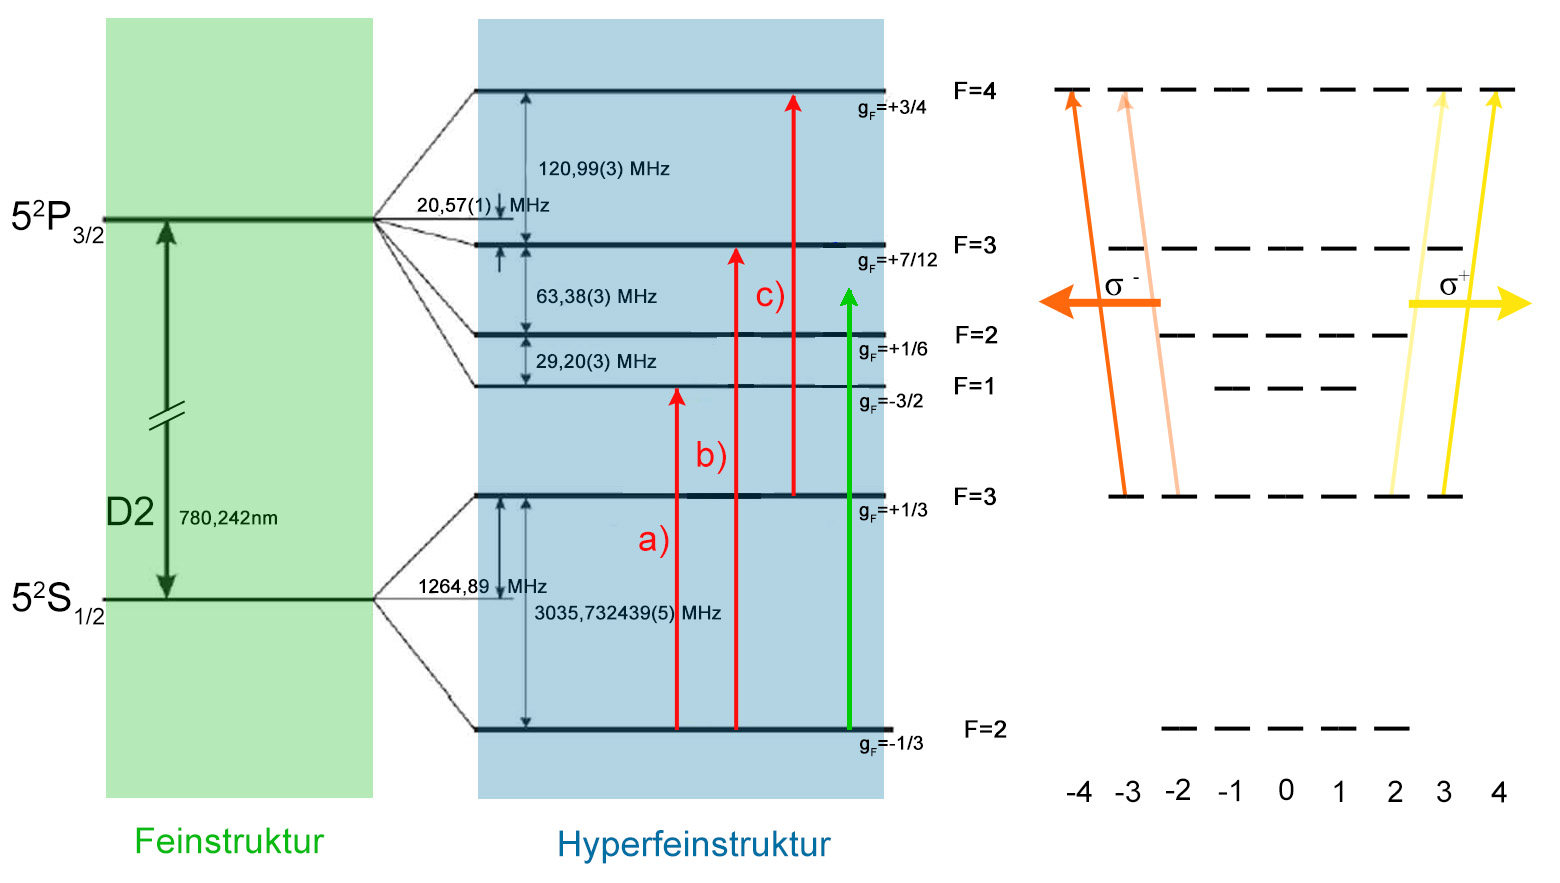
\includegraphics[width = 0.95\textwidth]{TS_korrigiert.jpg}
	\caption{Termschema D2-Linie inkl Laserlinien (a) Rückpumper Stabilisierung b) Rückpumper MOT c) Kühler MOT.}
\end{figure}

\newpage
\section*{Auswertung}
\subsection*{Eindimensionale Betrachtung}
Annahme: Gaußverteilung zu $t = 0$
\begin{align}
n(r, t= 0) \varpropto \exp\left(\frac{-x^2}{2 \sigma_x^2}\right)
\end{align}
Mit der eindimensionalen Geschwindigkeitsverteilung (Maxwell-Boltzmann) 
\begin{align}
g(v,T) = \left[\frac{m}{2 \pi k T}\right]^{\frac{1}{2}} \exp \left(\frac{-mv^2}{2kT}\right)
\end{align}
gilt dann zum Zeitpunkt $t>0$:
\begin{align}
n(r, t> 0) &\varpropto \int \mathrm{d}v \exp\left(\frac{-(x-vt)^2}{2 \sigma_x^2}\right) \cdot g(v,T) \\
&\varpropto \int \mathrm{d}v \exp\left(\frac{-(x-vt)^2}{2 \sigma_x^2}\right) \cdot \exp \left(\frac{-mv^2}{2kT}\right) \label{eq:falt} \\
&= \int \mathrm{d}v \exp\left(\frac{-x^2}{2 \sigma_x^2} + \frac{2xvt}{2 \sigma_x^2} - \frac{v^2 t^2}{2 \sigma_x^2} - \frac{mv^2}{2kT}\right) \\
&= \int \mathrm{d}v \exp\biggl(\frac{-x^2}{2 \sigma_x^2} + v \underbrace{\left( \frac{xt}{\sigma_x^2}\right)}_{b} - v^2 \underbrace{\left(\frac{t^2}{2 \sigma_x^2} + \frac{m}{2kT} \right)}_{a^2}\biggr) 
\end{align}
Bronstein, Wolfram o.ä. liefert:
\begin{align}
n(r, t> 0) &\varpropto \exp\left(\frac{-x^2}{2 \sigma_x^2}\right) \cdot \exp \left(\frac{b^2}{4a^2}\right) \\
&= \exp\left(\frac{-x^2}{2 \sigma_x^2}\right) \cdot \exp \left(\frac{\left( \frac{xt}{\sigma_x^2}\right)^2}{4\left(\frac{t^2}{2 \sigma_x^2} + \frac{m}{2kT} \right)}\right) \\
&= \exp\left(\frac{-x^2}{2 \sigma_x^2} + \frac{x^2t^2}{4\sigma_x^4\left(\frac{t^2}{2 \sigma_x^2} + \frac{m}{2kT} \right)}\right) \\
&= \exp\left(\frac{-x^2}{2 \sigma_x^2} + \frac{x^2t^2}{2\sigma_x^4\left(\frac{t^2}{\sigma_x^2} + \frac{m}{kT} \right)}\right) \\
&= \exp\left(\frac{-x^2 \cdot \sigma_x^2\left(\frac{t^2}{\sigma_x^2} + \frac{m}{kT} \right) +x^2t^2}{2\sigma_x^4\left(\frac{t^2}{\sigma_x^2} + \frac{m}{kT} \right)}\right) \\
&= \exp\left(\frac{-x^2 t^2 -  x^2 \sigma_x^2 \frac{m}{kT} +x^2t^2}{2\sigma_x^4\left(\frac{t^2}{\sigma_x^2} + \frac{m}{kT} \right)}\right) \\
&= \exp\left(\frac{- x^2 \sigma_x^2 \frac{m}{kT}}{2\sigma_x^4\left(\frac{t^2}{\sigma_x^2} + \frac{m}{kT} \right)}\right) \\
&= \exp\left(\frac{- x^2 \frac{m}{kT}}{2\sigma_x^2\left(\frac{t^2}{\sigma_x^2} + \frac{m}{kT} \right)}\right) \\
&= \exp\left(\frac{- x^2 \frac{m}{kT}}{2t^2 +2 \sigma_x^2 \frac{m}{kT} }\right) \\
&= \exp\left(\frac{- x^2 }{2\left(\frac{kT}{m}t^2 + \sigma_x^2\right)}\right) 
\end{align}
Die Atomdichte entspricht also wieder einer gaußschen Verteilung, allerdings mit breiteren Varianz
\begin{align}
\sigma_x^2 \left(t\right) = \frac{kT}{m}t^2 + \sigma_x^2 \label{final} 
\end{align}
Alternativ kann Gleichung \eqref{eq:falt} zu 
\begin{align}
n(r, t> 0) &\varpropto \int \mathrm{d}v \exp\left(\frac{-(\frac{x}{t}-v)^2}{2 \frac{\sigma_x^2}{t^2}}\right) \cdot \exp \left(\frac{-v^2}{2\frac{kT}{m}}\right) \\
\end{align}
umgeformt werden.
Hier ist die Faltung zweier Gaußverteilungen $g_1$ und $g_2$ im Sinne von
\begin{align}
g \left(\frac{x}{t}\right) = \left(g_1 * g_2\right) \left(\frac{x}{t}\right) = \int  g_1\left(\frac{x}{t}-v\right) g_2 \left(v\right)\mathrm{d}v
\end{align}
zu erkennen.
Diese Faltung ergibt bekanntermaßen wieder eine Normalverteilung.
Mit $\mu_1 = \mu_2 = 0$, $\sigma_1^2 = \frac{\sigma_x^2}{t^2}$ und $\sigma_2^2 = \frac{kT}{m}$ folgt dann für die Normalverteilung $g$:
\begin{align}
\mu &= \mu_1 + \mu_2 = 0 \\
\sigma^2 &= \sigma_1^2 + \sigma_2^2 =  \frac{\sigma_x^2}{t^2} + \frac{kT}{m}\\
\end{align}
Dies liefert mit 
\begin{align}
n(r, t> 0) &\varpropto \exp\left(\frac{\left(\frac{x}{t}\right)^2}{2 \sigma^2}\right) \\
&= \exp\left(\frac{x^2}{2 \sigma^2 t^2}\right) \\
&= \exp\left(\frac{- x^2 }{2\left(\frac{kT}{m}t^2 + \sigma_x^2\right)}\right) 
\end{align}
das gleiche Ergebnis (Gleichung \eqref{final}) wie obige Herleitung.
\end{document}